\section{Design Technique}
\label{sec:system_design}
The system design is a hardware/software co-design framework for low-power \gls{ml} analytics. This architecture allows design exploration for dedicated hardware accelerators in embedded systems. For \gls{ml} compatibility, the proposed framework integrates TensorFlow Lite Micro.

\subsection{Base Embedded System Architecture}
The embedded system architecture consists of a cooperative hardware-software platform. See \Fig{fig:system_architecture}. The embedded \gls{cpu} delegates low-level compute-bound tensor operations to the \glspl{tp}. The \glspl{tp} employ AXI-Lite interface for configuration and AXI-Stream interfaces via \gls{dma} for data movement from off-chip memory. Each \gls{tp} and \gls{dma} pair asserts interrupt flags once its compute job/transaction completes. Interrupt events are handled by the embedded \gls{cpu} to use the results and to start a new compute job/transaction. The hardware architecture can vary its resource utilization by customizing the \glspl{tp} prior to the hardware synthesis.
\begin{figure}[h!]
	\centering
	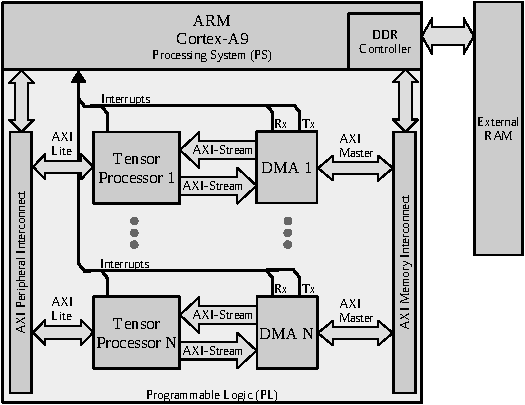
\includegraphics[width=0.5\textwidth]{./chapters/cnn_accelerator/figures/system_design.pdf}
	\caption{Base embedded system architecture.}
	\label{fig:system_architecture}
\end{figure}
\FloatBarrier
\subsection{Tensor Processor}
The \gls{tp} is a dedicated hardware module designed for the computation of tensor operations. This architecture employs AXI-Stream for high-performance communication with \gls{ram}, direct \gls{cpu} interface with AXI-Lite, and on-chip storage utilizing BRAM. Developed using \gls{hls}, its foundational tensor operations are based on the C++ TensorFlow Lite Micro kernels operators.  \Fig{fig:accelerator} provides a comprehensive visualization of the high-level hardware architecture.

Central to the design philosophy of the \gls{tp} is its adherence to the stationary weight taxonomy. This choice ensures that weights remain consistently stored in BRAM throughout computations. This strategy enhances performance by maximizing data reuse and minimizing data movement.

Operational efficiency is further achieved through a stream-oriented approach. In this paradigm, the \gls{tp} performs its processing as soon as the initial segment (receptive field) of the input tensor data is received. This ensures a continuous outflow of results, even before the complete input tensor is ingested. This operational approach reduces latency, aligning closely with the principles of the \gls{simd} category.
	
At the functional level, the \gls{tp} is designed for executing \textit{Conv2D} and \textit{DepthwiseConv2D} tensor operations, which are predominantly compute-bound tasks and constitute the computational backbone of \gls{ann}. The \gls{tp} supports both floating-point and fixed-point formats. Furthermore, its modular design allows the implementation of further tensor operations, enhancing its functionality and potential for future research.

This investigation concentrates on the custom floating-point \emph{Conv2D} tensor operation, this accelerates 2D convolution layers.

\begin{figure}[h!]
	\centering
	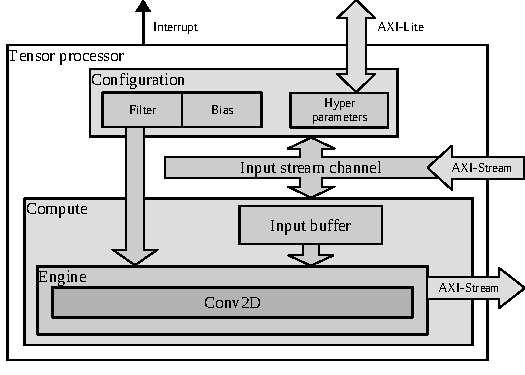
\includegraphics[width=0.5\textwidth]{./chapters/cnn_accelerator/figures/accelerator.pdf}
	\caption{High level hardware architecture of the proposed tensor processor.}
	\label{fig:accelerator}
\end{figure}
\FloatBarrier

\subsubsection{Modes of Operation}
The \gls{tp} functions in two primary modes: \textit{configuration} and \textit{execution}. The embedded \gls{cpu} establishes the mode of operation through the AXI-Lite interface. Each mode serves specific roles in the operation of the accelerator as detailed below:
\begin{itemize}
	\item \textbf{Configuration}: Here, the \gls{tp} first acquires a setup buffer detailing the tensor operation profile, including parameters such as stride, dilation, padding, offset, activation, quantized activation, depth-multiplier, tensor operation ID, and shapes for input, filter, bias, and output. The \gls{tp} then receives the filter and bias tensors, storing them in BRAM for both configuration and data reuse. These tensors are transferred in the standard \gls{fp} format, enveloping the 6-bit \gls{fp} representation, which the \gls{tp} extracts for optimized on-chip storage. During this phase, data is transferred from the off-chip DRAM to the on-chip BRAM, adhering to a stationary weight taxonomy.
	
	\Fig{fig:setup_transaction_chapter} illustrates the setup transaction buffer. Within the buffer, as shown in \Fig{fig:setup_transaction_chapter}(c), the tensor operator ID field indicates the type of operation, be it \textit{Conv2D} or \textit{DepthwiseConv2D}. \Fig{fig:sw_tp_delegate_job_chapter}(a) depicts the configuration mode and its associated setup buffer stream.
	
	\item \textbf{Execution}: In this mode, the \gls{tp} performs the tensor operation as dictated by the setup received in the previous configuration mode. During the execution of the tensor operation, input and output tensors are streamed using \gls{dma}. \Fig{fig:sw_tp_delegate_job_chapter}(b) highlights the execution mode, emphasizing the simultaneous movement of input and output tensor buffer streams. 
	During this phase, the \gls{tp} operates in a stream-oriented manner, performing the tensor operation as input tensor data is received and aligning with the \gls{simd} paradigm.
	

\end{itemize}


\begin{figure}[h!]
	\centering
	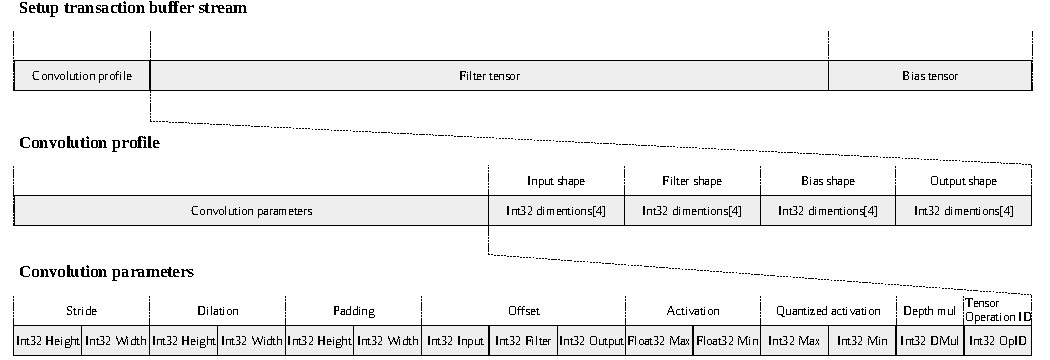
\includegraphics[width=\textwidth]{./figures/setup_transaction_buffer_stream.pdf}
	\caption{Setup transaction buffer stream.}
	\label{fig:setup_transaction_chapter}
\end{figure}

\begin{figure}[h!]
	\centering
	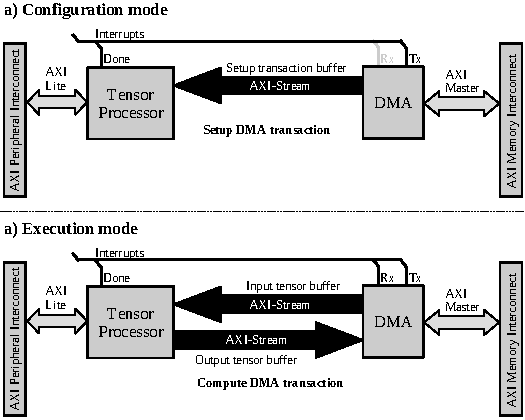
\includegraphics[width=0.5\textwidth]{./figures/task_execution.pdf}
	\caption{Tensor Processor task execution. (a) Depicts the configuration mode along with its corresponding setup buffer stream. (b) Illustrates the execution mode, showcasing concurrent input and output tensor buffer streams.}
	\label{fig:sw_tp_delegate_job_chapter}
\end{figure}


\FloatBarrier
\subsubsection{Dot-product with Hybrid Floating-Point}
\label{sec:dot_product}
It is implemented the floating-point computation adopting the dot-product with hybrid custom floating-point~\cite{nevarez2021accelerating}. The hardware dot-product is illustrated in \Fig{fig:dot_product} and \Fig{fig:dot_product_loop}(a). This design instantiates a \gls{hf6} \gls{mac} with an internal accumulator register of 64-bit fixed-point with 23-bit fraction. During operation, the feature map and filter values are extracted from on-chip memory (BRAM). Both values have to be different than zero to enable the \gls{mac} operation. The result is biased by accumulating a denormalized bias value. Since the bias is stored with 6-bit \gls{fp}, its fractional part has to be aligned with the 23-bit fraction of the accumulator, see \Fig{fig:dot_product_loop}(b). The ReLu activation is applied to the accumulator and its result is normalized to convert it to IEEE 754 standard \gls{fp}, see \Fig{fig:dot_product_loop}(c).

Rather than a parallelized hardware structure, this approach is a pipelined hardware design suitable for resource-limited devices. The latency in clock cycles of this hardware module is defined by \equ{eq:dot_custom_float_latency}, where $N$ is the length for the vector dot-product. This latency equation is obtained from the general pipelined hardware latency formula: $L=\left(N-1\right)II+IL$, where $II$ is the initiation interval, and $IL$ is the iteration latency. Both $II$ and $IL$ are obtained from the \gls{hls} results. Both the exponent and mantissa bit widths of the filter and bias are set to 4-bit exponent and 1-bit mantissa (E4M1), which corresponds to float6 quantization.

\begin{eqnarray} \label{eq:dot_custom_float_latency}
L_{hf}=N+7
\end{eqnarray}

\begin{figure}[h!]
	\centering
	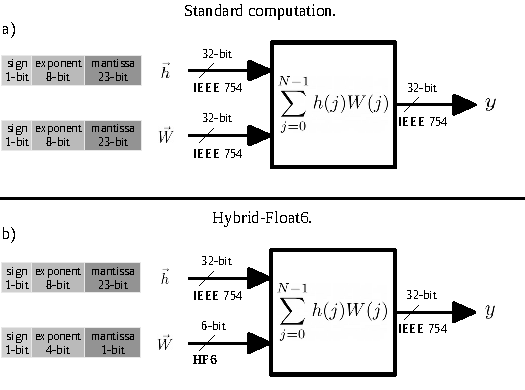
\includegraphics[width=0.5\textwidth]{./chapters/cnn_accelerator/figures/dot-product_unit.pdf}
	\caption{Dot-product hardware module with (a) standard floating-point and (b) Hybrid-Float6.}
	\label{fig:dot_product}
\end{figure}

\begin{figure}[h!]
	\centering
	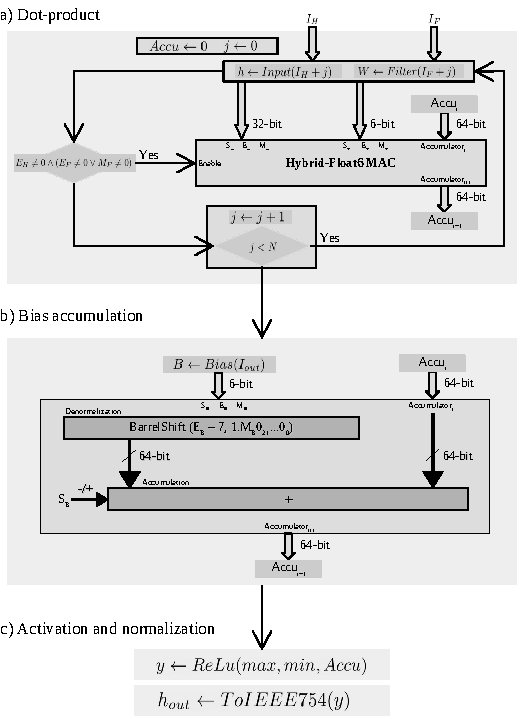
\includegraphics[width=0.5\textwidth]{./chapters/cnn_accelerator/figures/dot_product_hybrid.pdf}
	\caption{(a) Dot-product hardware module with Hybrid-Float6 MAC, (b) bias accumulation, (c) activation and normalization to IEEE754.}
	\label{fig:dot_product_loop}
\end{figure}

\subsubsection{Multiply-Accumulate Unit}
The multiply-accumulate operation calculates the product of two numbers and adds the result to an accumulator. In \gls{fp} arithmetics, the area of a hardware multiplier scales with the bit size of the mantissas. In the case of \gls{hf6}, the 6-bit \gls{fp} representation allows a reduced hardware multiplicator for mantissas. The 1-bit mantissa enables optimized \gls{mac} implementations by reducing the mantissa multiplication to a multiplexed addition, see \fig{fig:multiplier}. This \gls{mac} produces denormalized results, which are accumulated in a fixed-point accumulator. This approach reduces latency, energy consumption, and hardware area/resource utilization.

\begin{figure}[h!]
	\centering
	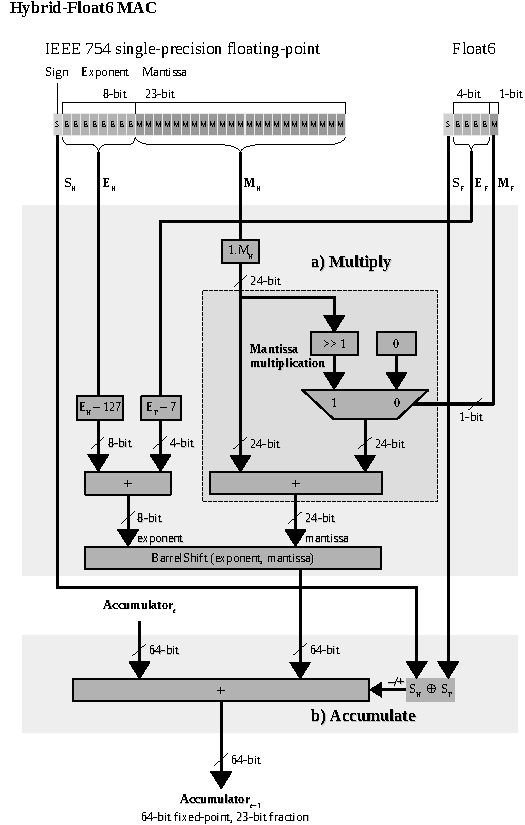
\includegraphics[width=0.5\textwidth]{./chapters/cnn_accelerator/figures/multiplier.pdf}
	\caption{Hybrid-Float6 multiply-accumulate hardware design.}
	\label{fig:multiplier}
\end{figure}

Special cases, such as Infinity and \gls{nan}, are not considered in this design for simplicity, since they are not expected for \gls{cnn} inference. For the subnormal case, the element-wise multiplication is disabled when having a zero entry and approximated when having subnormal mantissa. The feature map values are considered zero when the exponent is zero ($E_H=0$). The filter values are considered zero when both exponent and mantissa are zero ($E_F=0\land M_F=0$). See \Fig{fig:dot_product_loop}(a). In the 6-bit \gls{fp}, the 1-bit mantissa has one subnormal case, which is handled as a normalized case. This exploits the intrinsic error tolerance to reduce the hardware design.

The approximation error is defined by the difference between \Equ{eq:float} and \Equ{eq:float_subnorm} when $E=0$ and $M=2^{-1}$. The result defines the error as $e=2^{-B-1}$. Then, from \Equ{eq:float_bias} with $E_{size}=4$, gives $B=7$. Hence, $e=3.9\mathrm{e}{-3}$. This error is produced when having the subnormal case $E=0$ and $M=2^{-1}$, which corresponds to the value $\pm7.8\mathrm{e}{-3}$ deviated to $\pm1.17\mathrm{e}{-2}$. This approximation leverages the intrinsic error tolerance of \gls{cnn} to reduce hardware resource utilization and energy consumption~\cite{du2014leveraging}.


\subsubsection{On-chip Memory Utilization}
\label{sec:memory_utilization}
The total on-chip memory utilization on the \gls{tp} is defined by \Equ{eq:tp_memory}, where $TP_B$ and $V_{M}$ represent the tensor buffers required for \emph{Conv} operation and local registers required for the logic, respectively. \Equ{eq:tp_memory_buffer} defines the tensor buffers, where $Input_{M}$ is the \emph{input buffer}, $Filter_{M}$ is the \emph{filter buffer}, $Bias_{M}$ is the \emph{bias buffer}. These on-chip memory buffers are defined in bits. \fig{fig:accelerator_buffers} illustrates the convolution operation utilizing the on-chip memory buffers.
\begin{figure}
	\centering
	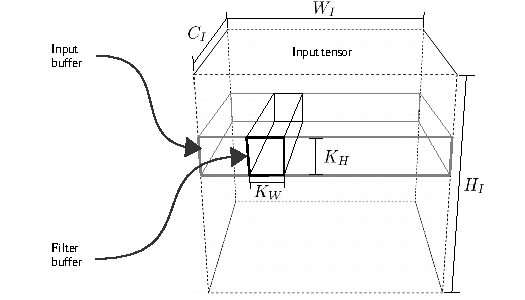
\includegraphics[width=0.5\textwidth]{./chapters/cnn_accelerator/figures/accelerator_buffers.pdf}
	\caption{Design parameters for on-chip memory buffers on the TP.}
	\label{fig:accelerator_buffers}
\end{figure}
\begin{eqnarray} \label{eq:tp_memory}
TP_{M}=TP_B+V_{M}
\end{eqnarray}
\begin{eqnarray} \label{eq:tp_memory_buffer}
TP_{B}=Input_{M}+Filter_{M}+Bias_{M}
\end{eqnarray}

The memory utilization of \emph{input buffer} is defined by \Equ{eq:input_memory}, where $K_{H}$ is the height of the convolution kernel, $W_{I}$ is the width of the input tensor (input feature maps), $C_{I}$ is the number of input channels, and $BitSize_{I}$ is the bit size representation used by the input tensor.
\begin{eqnarray} \label{eq:input_memory}
Input_{M}=K_{H}W_{I}C_{I}BitSize_{I}
\end{eqnarray}

The memory utilization of \emph{filter buffer} is defined by \Equ{eq:filter_memory}, where $K_{W}$ and $K_{H}$ are the width and height of the convolution kernel, respectively; $C_{I}$ and $C_{O}$ are the number of input and output channels, respectively; and $BitSize_{F}$ is the bit size representation used by filter values.
\begin{eqnarray} \label{eq:filter_memory}
Filter_{M}=C_{I}K_{W}K_{H}C_{O}BitSize_{F}
\end{eqnarray}

The memory utilization of \emph{bias buffer} is defined by \Equ{eq:bias_memory}, where $C_{O}$ is the number of output channels, and $BitSize_{B}$ is the bit size representation used by bias values.
\begin{eqnarray} \label{eq:bias_memory}
Bias_{M}=C_{O}BitSize_{B}
\end{eqnarray}

As a design trade-off, \Equ{eq:channel_in_memory} defines the capacity of output channels based on given design parameters. The total on-chip memory $TP_{M}$ determines the \gls{tp} storage capacity.
\begin{eqnarray} \label{eq:channel_in_memory}
C_{O}=\frac{TP_{M}-V_{M}-K_{H}W_{I}C_{I}BitSize_{I}}{C_{I}K_{W}K_{H}BitSize_{F}+BitSize_{B}}
\end{eqnarray}

The floating-point formats implemented in the \gls{tp} are defined by $BitSize_F$, $BitSize_B$ and $BitSize_I$. The HF6 defines 6-bit for $BitSize_F$ and $BitSize_B$, and 32-bit for $BitSize_I$. These are design parameters defined before hardware synthesis. This allows fine control of BRAM utilization, which is suitable for resource-limited devices.
\FloatBarrier
\subsection{Training Method}
The training method consists of two separate stages: (1) training with iterative early stop and (2) quantization-aware training.
 
\subsubsection{Training with Iterative Early Stop}
To achieve better performance on \gls{cnn}-regression models, it is implemented a training procedure with iterative early stop cycle. This allows to reach better local minima. This process consists of four steps:

\begin{enumerate}
	\item A model is obtained with an initial training with standard early stop monitoring.
	\item The model is iteratively re-trained (refined) with standard early stop. This process iteratively restarts the moving averages of the optimizer to search for better local minima.
	\item In case of a better local minimum, the model is saved and used as a base for subsequent search iterations, otherwise it is a discarded search.
	\item The cyclic process stops automatically with a given number of searches without a better local minimum, this number of searches is denoted as the \textit{stop patience}. This allows to set a maximum number of unsuccessful search trials before the stop.
\end{enumerate}

This method is described in \Algo{alg:training}.

\subsubsection{Quantization-Aware Training}
The \gls{qat} method is integrated into the training process, this operates as a callback on each mini-batch update. The quantization is applied on the trainable parameters of convolution layers. This method is implemented on the \gls{ml} framework (TensorFlow/Keras), see \Algo{alg:quantization_integration}.

The quantization method uses rounding strategy to reduce the \gls{fp} representation. This maps the full precision \gls{fp} values to the closest representable 6-bit \gls{fp} values, see \Algo{alg:quantize_training}. This method quantizes the filter and bias tensors of the convolution layers. The exponent bit size plays a more predominant influence on the model accuracy than the mantissa bit size. In \cite{lai2017deep}, Lai \textit{et al.} demonstrated that 4-bit exponent and X-bit mantissa is adequate and consistent across different networks (SqueezeNet, AlexNet, GoogLeNet, VGG-16). In this research, the \gls{fp} representation with 4-bit exponent and 1-bit mantissa is investigated.

\begin{algorithm}[h!]
	\caption{Training with iterative early stop cycle.}
	\label{alg:training}
	\begin{algorithmic}
		\SetAlgoLined
		\renewcommand{\algorithmicrequire}{\textbf{input:}}
		\renewcommand{\algorithmicensure}{\textbf{output:}}
		\REQUIRE $MODEL$ as the input model.
		\REQUIRE $D_{train}$ as the training data set.
		\REQUIRE $D_{val}$ as the validation data set.
		\REQUIRE $N_{I}$ as the stop patience for iterative training cycle.
		\REQUIRE $N_{E}$ as the early stop patience (epochs) for training.
		\REQUIRE $B_{size}$ as the mini-batch size.
		\ENSURE $MODEL$ as the full-precision output model.
		\STATE $Train(MODEL, D_{train}, D_{val}, N_{E}, B_{size})$
		\STATE $mse_i \gets Evaluate(MODEL, D_{val})$ // Benchmark
		\STATE $n_I \gets 0$
		\WHILE {$n_I<N_I$}
		\STATE // Iterative early stop cycle
		\STATE $Train(MODEL, D_{train}, D_{val}, N_{E}, B_{size})$
		\STATE $mse_v \gets Evaluate(MODEL, D_{val})$
		\IF{$mse_v < mse_i$}
			\STATE $Update(MODEL)$
			\STATE $mse_i \gets mse_v$
		\ELSE
			\STATE $MODEL  \gets LoadPreviousWeights()$
			\STATE $n_I \gets n_I + 1$
		\ENDIF
		\ENDWHILE
	\end{algorithmic}
\end{algorithm}


\begin{algorithm}[h!]
	\caption{OnMiniBatchUpdate\_Callback.}
	\label{alg:quantization_integration}
	\begin{algorithmic}
		\SetAlgoLined
		\renewcommand{\algorithmicrequire}{\textbf{input:}}
		\renewcommand{\algorithmicensure}{\textbf{output:}}
		\REQUIRE $MODEL$ as the full-precision input model.
		\REQUIRE $E_{size}$ as the target exponent bits size.
		\REQUIRE $M_{size}$ as the target mantissa bits size.
		\REQUIRE $D_{train}$ as the training data set.
		\REQUIRE $D_{val}$ as the validation data set.
		\REQUIRE $N_{ep}$ as the number of epochs.
		\REQUIRE $B_{size}$ as the mini-batch size.
		\ENSURE $MODEL$ as the quantized output model.
		\STATE // Quantize
		\STATE $MODEL \gets$ \Algo{alg:quantize_training}$(MODEL,E_{size}, M_{size})$ 
		\IF {$1<epoch$}
		\STATE // Update model after first epoch
		\STATE $mse_v \gets Evaluate(MODEL, D_{val})$
		\IF{$mse_v < mse_i$}
		\STATE $Update(MODEL)$
		\STATE $mse_i \gets mse_v$
		\ENDIF
		\ENDIF
	\end{algorithmic}
\end{algorithm}

\begin{algorithm}[h!]
	\caption{Custom floating-point quantization.}
	\label{alg:quantize_training}
	\begin{algorithmic}
		\SetAlgoLined
		\renewcommand{\algorithmicrequire}{\textbf{input:}}
		\renewcommand{\algorithmicensure}{\textbf{output:}}
		\REQUIRE $MODEL$ as the CNN.
		\REQUIRE $E_{size}$ as the target exponent bit size.
		\REQUIRE $M_{size}$ as the target mantissa bits size.
		\REQUIRE $STDM_{size}$ as the IEEE 754 mantissa bit size.
		\ENSURE $MODEL$ as the quantized CNN.
		\FOR {$layer$ in $MODEL$}
		\IF {$layer$ is $Conv2D$ or $SeparableConv2D$}
		\STATE $filter, bias \gets GetWeights(layer)$
		\FOR {$x$ in $filter$ and $bias$}
			\STATE $sign \gets GetSign(x)$
			\STATE $exp \gets GetExponent(x)$
			\STATE $fullexp \gets 2^{E_{size}-1}-1$ // Get full range value
			\STATE $cman \gets GetCustomMantissa(x, M_{size})$
			\STATE $leftman \gets GetLeftoverMantissa(x, M_{size})$
			\IF {$exp <-fullexp$}
				\STATE$x\gets0$
			\ELSIF{$exp > fullexp$}
				\STATE$x\gets (-1)^{sign}\cdot2^{fullexp}\cdot(1+(1-2^{-M{size}}))$
			\ELSE
				\IF {$2^{STDM_{size}-M_{size}-1}-1<leftman$}
					\STATE $cman \gets cman+1$ // Above halfway
					\IF{$2^{M_{size}}-1<cman$}
					\STATE $cman \gets 0$ // Correct mantissa overflow
					\STATE $exp \gets exp + 1$
					\ENDIF
				\ENDIF
				\STATE // Build custom quantized floating-point value
				\STATE$x\gets (-1)^{sign}\cdot2^{exp}\cdot(1+cman\cdot2^{-M_{size}})$
			\ENDIF
		\ENDFOR
		\STATE $SetWeights(layer, filter, bias)$
		\ENDIF
		\ENDFOR
	\end{algorithmic}
\end{algorithm}

\FloatBarrier
\subsection{Embedded Software Architecture}
The software architecture is a layered object-oriented application framework written in C++, see \fig{fig:sw_stack} and \fig{fig:sw_stack_flowchart}. Description of the software layers is as follows:
\begin{itemize}
	\item \textbf{Application}: As the highest level of abstraction, this software layer implements the analytics application, this invokes the \gls{ml} library.
	\item \textbf{Machine Learning Library}: This software layer offers a comprehensive high level \gls{api} for \gls{ml} inference. This layer consist of TensorFlow Lite Micro, this is modified to implement the delegate software interfaces for the proposed hardware accelerator.
	\item \textbf{Hardware Abstraction Layer}: This layer consist of the hardware drivers used in the TFLite delegate interfaces. This software layer handles initialization and runtime operation of the \gls{tp} and \gls{dma}.
\end{itemize}

\begin{figure}[h!]
	\centering
	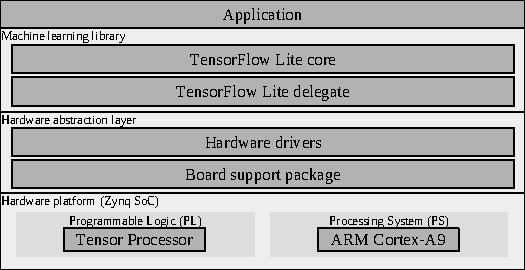
\includegraphics[width=0.5\textwidth]{./chapters/cnn_accelerator/figures/sw_stack.pdf}
	\caption{High level embedded software architecture.}
	\label{fig:sw_stack}
\end{figure}

\begin{figure}[h!]
	\centering
	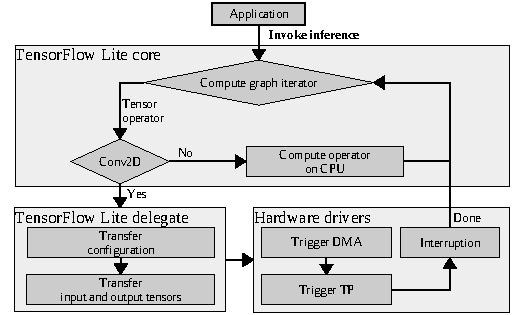
\includegraphics[width=0.5\textwidth]{./chapters/cnn_accelerator/figures/sw_stack_flowchart.pdf}
	\caption{Software flowchart.}
	\label{fig:sw_stack_flowchart}
\end{figure}

\paragraph{Model Deployment}

In TensorFlow, model creation, training, and evaluation typically proceed through the use of the Keras API. Once the model has been evaluated for performance, there are two primary methods for deployment:

\begin{itemize}
	\item \textbf{SD Card Method:} The trained model is saved in the .tflite format and stored on an SD card. This card is then inserted into the \gls{soc} \gls{fpga} slot.
	
	\item \textbf{Embedded Software Method:} Alternatively, the model can be embedded directly into the code of the embedded software by converting it into a hex dump (using xxd tool). This is then compiled into the application, eliminating the need for external storage.
\end{itemize}

This dual-method approach provides flexibility for a range of deployment scenarios.


%%%%%%%%%%%%%%%%%%%%%%%%%%%%%%%%%%%%%%%%%%%%%%%%%%%%%%%%%%%%
\subsubsection{TensorFlow Lite Delegate Implementation and Operation}
TensorFlow, as an open-source framework, provides extensible interfaces to optimize the execution of specific parts of a model on various hardware types. Within this structure, delegates are components that help TensorFlow Lite to efficiently reroute specific tensor operations to be run on specialized hardware accelerators, rather than the default \gls{cpu}.


\paragraph{Implementation}

In the TensorFlow ecosystem, a delegate serves as a bridge connecting hardware and software, illustrated in \Fig{fig:sw_stack}. In this framework, specific tensor operations are offloaded to specialized hardware like \glspl{gpu}, \glspl{npu}, and custom accelerators such as the \gls{tp}. To harness the full potential of the proposed \gls{tp}, it is needed to implement a tailored TensorFlow Lite delegate.

The delegate interface identifies operations eligible for offloading and redirects them to the specialized hardware, as depicted in \Fig{fig:sw_stack_flowchart}.

\paragraph{Software Classes}

The collaboration diagram in \Fig{fig:sw_tp_delegate_diagram} offers a visual representation of the relationships between the delegate class implemented for the \gls{tp}. This diagram is instrumental in understanding the interactions between classes and can be insightful for developers and researchers who aim to customize or extend the TensorFlow Lite delegate for specialized use-cases.

In this diagram, the central class is the \textit{TPDelegate}, representing the delegate designed for the proposed custom \gls{tp}. This delegate interacts with a variety of other classes, facilitating execution of tensor operations and its memory/hardware management.

\begin{figure}[h!]
	\centering
	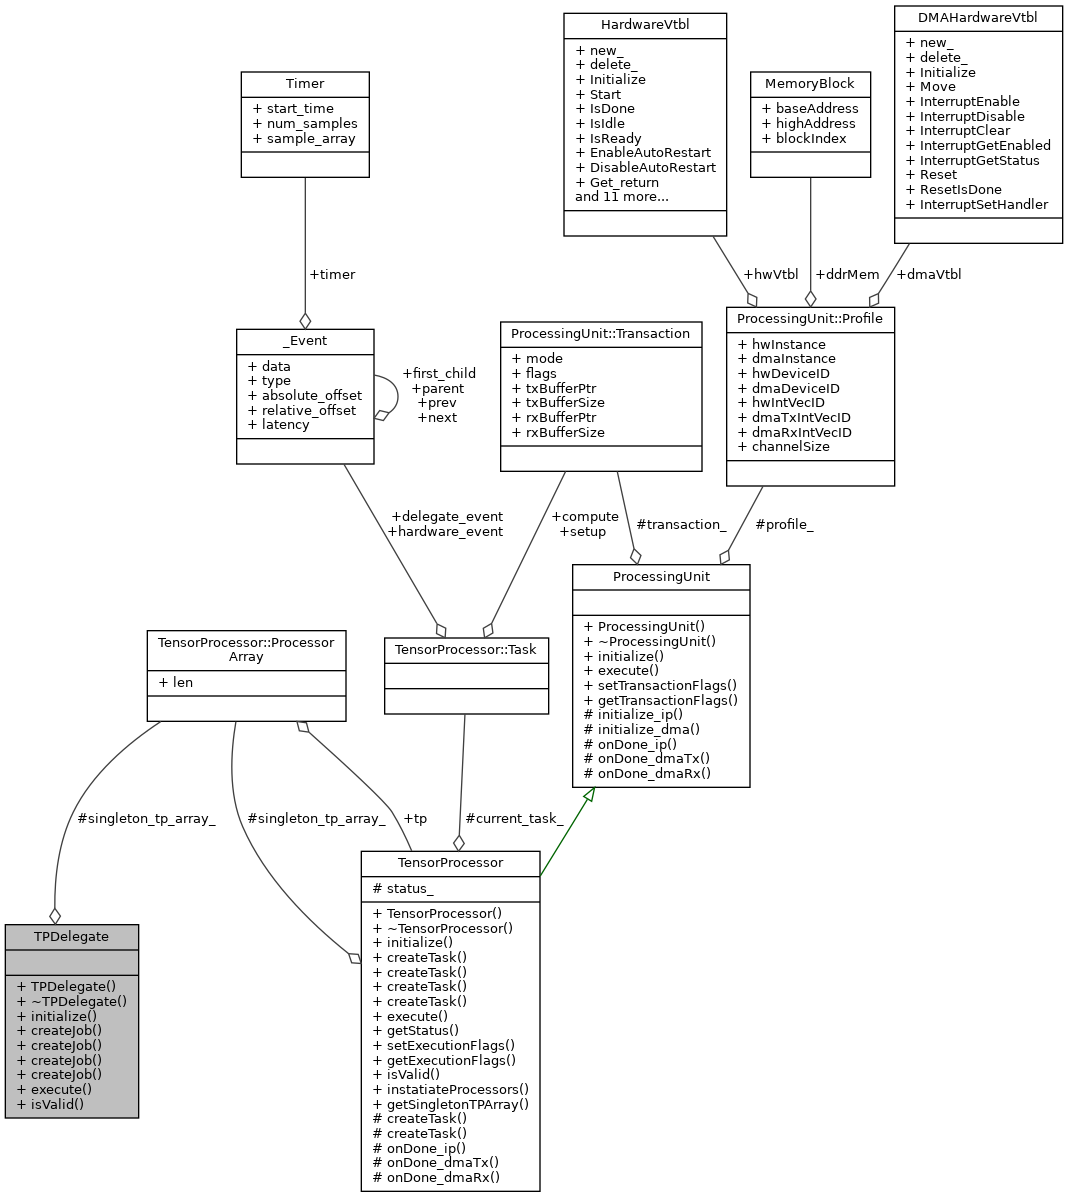
\includegraphics[width=\textwidth]{./figures/class_t_p_delegate__coll__graph.png}
	\caption{Collaboration diagram of TensorFlow delegate classes.}
	\label{fig:sw_tp_delegate_diagram}
\end{figure}
\FloatBarrier

\paragraph{Initialization}

As depicted in \Fig{fig:sw_tf_delegate_initialize_diagram}, the process commences by enabling the delegate interface at the application layer. Subsequently, the \textit{MicroInterpreter} module creates and initializes a \textit{TPDelegate} instance. During this phase, the \gls{tp} and \gls{dma} hardware drivers are also instantiated and initialized.

\begin{figure}[h!]
	\centering
	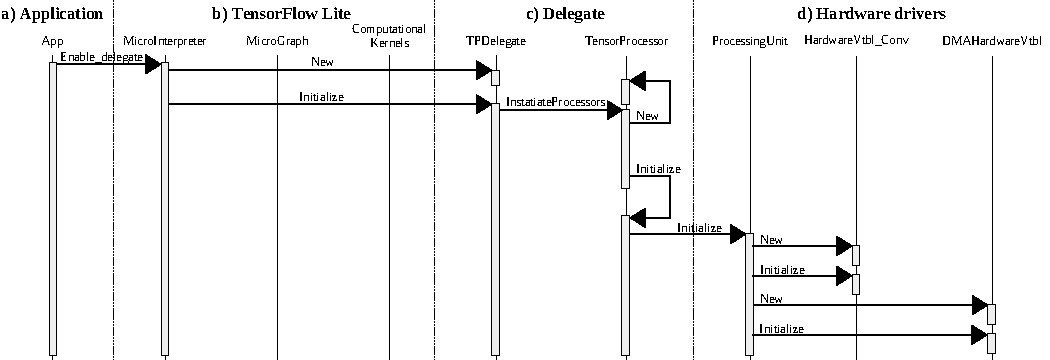
\includegraphics[width=\textwidth]{./figures/sequence_tfl_delegate_initialization.pdf}
	\caption{Sequence diagram of TensorFlow delegate initialization.}
	\label{fig:sw_tf_delegate_initialize_diagram}
\end{figure}
\FloatBarrier

\paragraph{Operation}
During operation, TensorFlow Lite executes the model graph. Essentially, this graph provides a representation of how data is processed and transformed as it moves through the various operations of a \gls{ml} model. 
The execution of the computation graph is depicted in \Fig{fig:sw_tf_delegate_execution_diagram}. Called by the application layer, the \textit{MicroInterpreter} module invokes the subgraph execution. As depicted in \Fig{fig:sw_stack_flowchart}, the process involves the following steps:

\begin{enumerate}
	\item Traversing through each node in the compute graph.
	\item Assessing the tensor operator of each node and delegating the computation of \textit{Conv2D} operations to the \gls{tp}.
\end{enumerate}

\begin{figure}[h!]
	\centering
	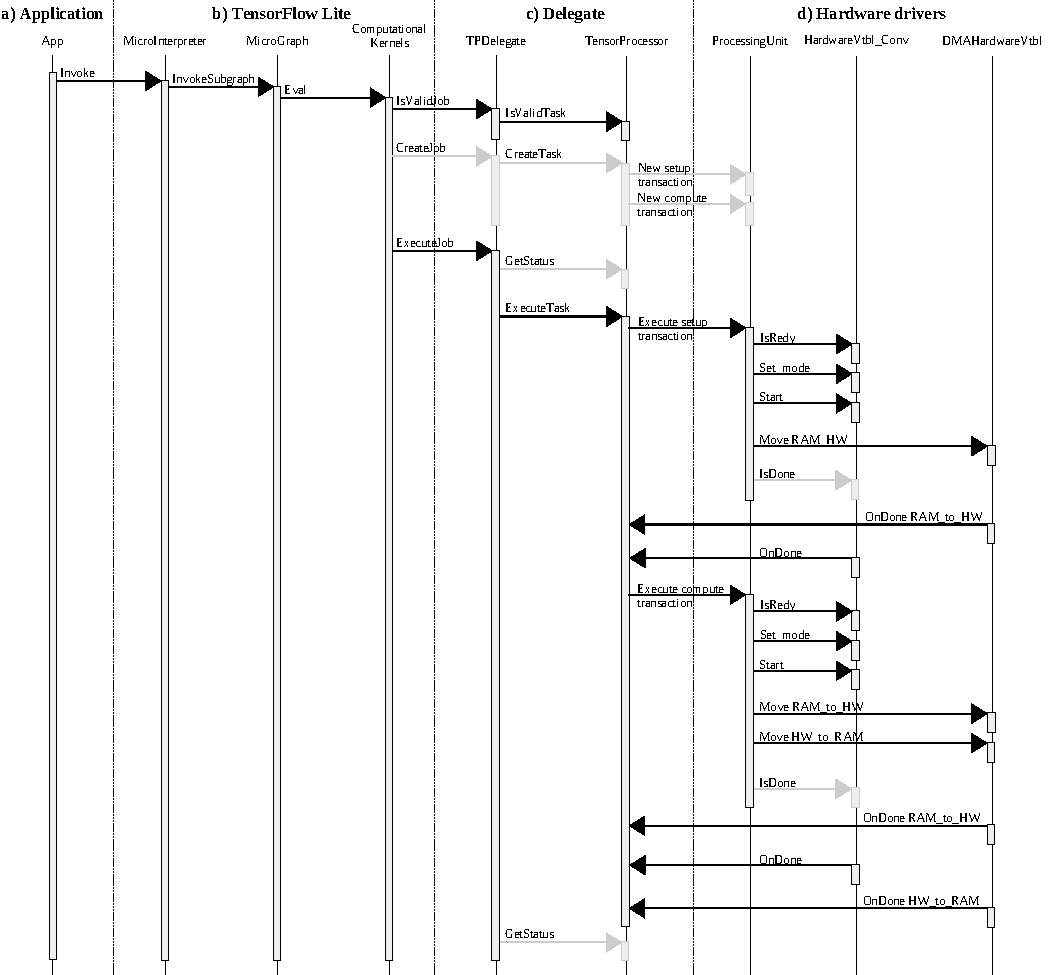
\includegraphics[width=\textwidth]{./figures/sequence_tfl_delegate_acceleration.pdf}
	\caption{Sequence diagram of TensorFlow delegate execution.}
	\label{fig:sw_tf_delegate_execution_diagram}
\end{figure}

When the delegate operates the \gls{tp}, it creates a \textit{Job} object that serves as a tasks container for the \gls{tp}. In this case, it contains \textit{Conv2D} operation task. Each task contains two data transactions:

\begin{itemize}
	\item \textbf{Setup Transaction:} Here, the \gls{dma} transfers the setup buffer (as depicted in \Fig{fig:setup_transaction_chapter}) from its memory source to the \gls{tp}, to establish a groundwork for the upcoming \textit{Conv2D} execution. Refer to \Fig{fig:sw_tp_delegate_job_chapter}(a). During this transaction, the \gls{tp} operates in its \textit{configuration} mode.
	\item \textbf{Compute Transaction:} As the core of the operation, the input tensor gets streamed to the \gls{tp} via the \gls{dma} TX channel from its memory source. Concurrently, the output tensor flows out from the \gls{tp}, to its memory destination through the \gls{dma} RX channel. Refer to \Fig{fig:sw_tp_delegate_job_chapter}(b). During this transaction, the \gls{tp} operates in its \textit{execution} mode.
\end{itemize}

The TensorFlow Lite delegate implementation encapsulates the mechanisms of software-hardware synergy, pushing the efficient neural network execution on custom hardware platforms.

Details on the delegate interface implementation and associated hardware drivers are provided in Appendix~\ref{chap:appendix_delegate}, while modifications to TensorFlow Lite library are presented in Appendix~\ref{chap:code_changes}.
\FloatBarrier